\chapter{Historical Development}\label{ch:historical_development}

In the early 20th century, as urbanization accelerated and automobile ownership increased, the need for efficient parking solutions became apparent. The first significant step in this direction came in 1905 with the Garage Rue de Ponthieu \autocite{mcdonald2005parking} in Paris, designed by Auguste Perret. This multi-story concrete structure, see \cref{fig:garage_rue_de_ponthieu}, featured internal elevators to transport cars between floors, where attendants would manually park them. While not fully automated, this innovation laid the foundation for future parking systems by maximizing vertical space utilization.

The 1920s marked the beginning of more advanced parking solutions, particularly in major U.S. cities. The Paternoster system \autocite{paternoster2022}, resembling a Ferris wheel for cars, refer to \cref{fig:pater_noster_parking_system}, could accommodate eight vehicles in the space typically used for two. This period also saw the introduction of Kent Automatic Garages in New York in 1928, which employed an electric "parker" to lift and move cars to available spaces. These early automated systems represented significant progress in addressing the growing demand for parking in densely populated urban areas.

\begin{figure}
	\hfill
	\begin{subfigure}{0.45\textwidth}
		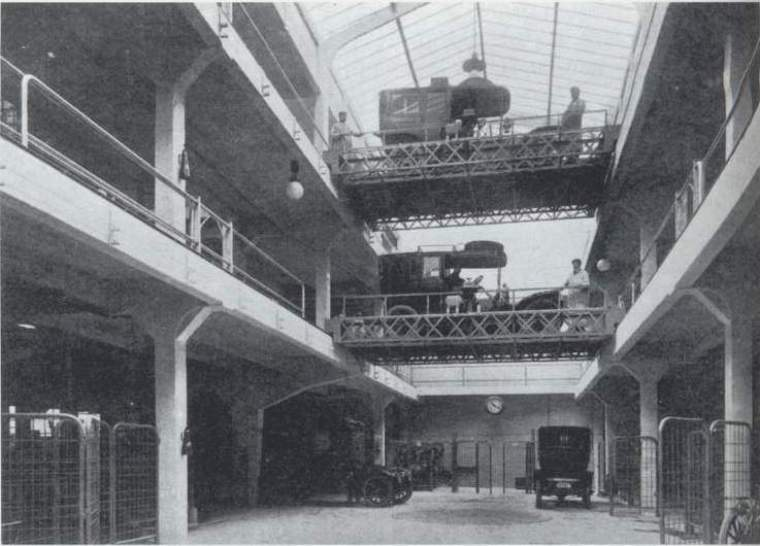
\includegraphics{garage_du_rue_ponthieu.jpg}
		\caption{Garage Rue de Ponthieu in Paris, 1905 \autocite{mcdonald2005parking}.}\label{fig:garage_rue_de_ponthieu}
	\end{subfigure}
	\hfill
	\begin{subfigure}{0.45\textwidth}
		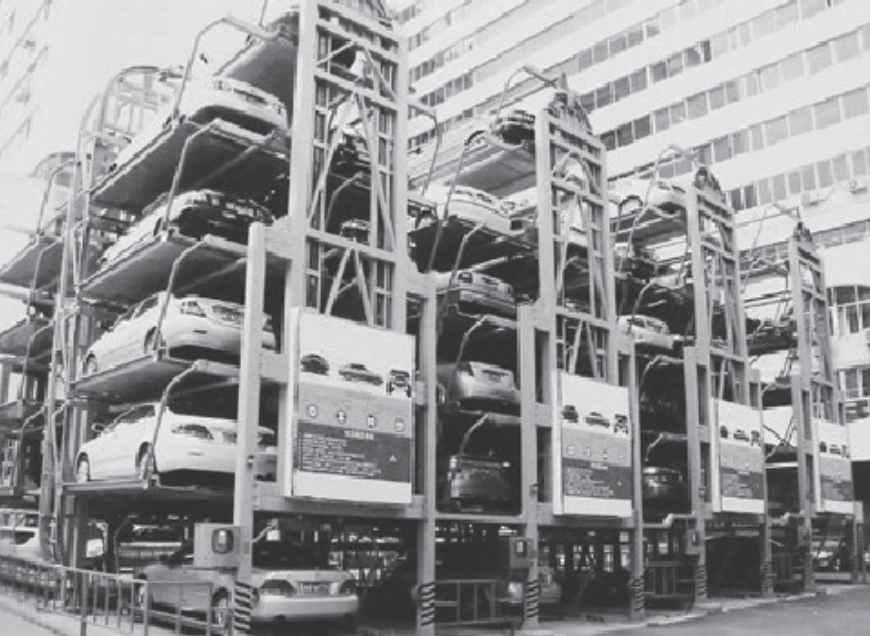
\includegraphics{paternoster.png}
		\caption{Paternoster system, 1920s \autocite{paternoster2022}.}\label{fig:pater_noster_parking_system}
	\end{subfigure}
	\hfill

	\caption{Historical developments in parking management systems.}
\end{figure}

The 1930s brought another crucial development with the introduction of parking meters, revolutionizing on-street parking management. This innovation allowed cities to better regulate parking durations and generate revenue from public parking spaces. The subsequent decades, particularly the 1940s and 1950s, witnessed a surge in the development of automated parking systems in the United States, with designs such as Bowser, Pigeon Hole, and Roto Park \autocite{shoup2012cars} gaining popularity.

While interest in automated parking systems temporarily waned in the U.S. during the 1960s to 1980s, development continued in Europe and Asia. Notable advancements included the Auto Stacker system in London in 1961 and Wohr's Electromechanical Parking System Type 100 \autocite{hardingaps2021history} in Germany in 1962. During this period, Japan emerged as a leader in automated parking systems, with significant growth continuing into the 1990s.

The late 20th century marked the beginning of the digital revolution in parking management. The 1990s saw the introduction of parking guidance systems, which used sensors to monitor occupancy and provide real-time information to drivers. This technology significantly reduced the time and frustration associated with finding available parking spaces in large facilities.

The early 2000s ushered in a new era of smart parking solutions. In 2002, the first robotic parking garage in the United States opened in Hoboken, New Jersey \autocite{usatoday2007robotic}, showcasing the potential of fully automated parking facilities. This period also saw the rapid development of technologies such as license plate recognition systems, mobile parking apps for finding and reserving spaces, and IoT-based parking management systems.

In recent years, parking management systems have continued to evolve, incorporating advanced technologies such as artificial intelligence and machine learning for predictive parking analytics. Cloud-based parking management platforms have become increasingly common, offering scalable and flexible solutions for parking operators. Furthermore, the integration of parking systems with broader smart city initiatives and connected vehicle technologies is paving the way for more efficient and sustainable urban mobility solutions.

The evolution of parking management systems reflects broader technological trends, moving from mechanical solutions to digital, interconnected systems. Today's parking management solutions prioritize efficiency, user experience, and environmental sustainability, addressing not only the immediate needs of drivers and parking operators but also contributing to the broader goals of smart urban planning and reduced environmental impact.

As cities continue to grow and evolve, parking management systems will undoubtedly play a crucial role in shaping the future of urban mobility. The ongoing development of these systems promises to further optimize space utilization, reduce traffic congestion, and enhance the overall urban experience for residents and visitors alike.
